\documentclass[11pt]{article}
\usepackage[review]{acl}
\usepackage{times}
\usepackage{latexsym}
\usepackage[T1]{fontenc}
\usepackage[utf8]{inputenc}
\usepackage{microtype}
\usepackage{inconsolata}
\usepackage{graphicx}
\usepackage{enumitem}
\usepackage{booktabs}
\usepackage{amsmath}
\usepackage{amssymb}
\usepackage{xcolor}
\usepackage{tikz}
\usetikzlibrary{arrows.meta,positioning,fit,backgrounds}

% colorblind-safe palette (Wong 2011), shared with figs/make_*.py
\definecolor{cbBlue}{RGB}{0,114,178}
\definecolor{cbOrange}{RGB}{213,94,0}
\definecolor{cbGreen}{RGB}{0,158,115}
\definecolor{cbGray}{RGB}{120,120,120}

\newcommand{\rtwo}{$R^2$}
\newcommand{\bc}{$B\!\cdot\!C$}

\title{A Dormant Subspace, Not a Missing One: A Decodable but Causally\\ Inert Answer-Site Representation of Arithmetic in Llama-3.1-8B}

\author{Anonymous ACL submission}

\begin{document}
\maketitle

\begin{abstract}
Large language models often fail at arithmetic composition even when they solve
every part in isolation. We study a token-matched instance in Llama-3.1-8B:
wrapping a multiplicative operand in an additive identity, $(\,0 + B\,) * C$,
collapses multiplication accuracy (instruct $0.27$, base $0.51$) although the model
evaluates the wrapped sub-expression perfectly ($1.00$) and multiplies inside a
bracket ($0.91$). The failure is operation-specific (the additive analogue composes
at $0.99$), depth-sensitive, magnitude-controlled, and recovers with a few in-context
examples. We then ask what the internal representation looks like. At the answer
position the operand $B$ and the near-product \bc{} are linearly decodable
($R^2 \approx 0.96$), which invites a ``the value is there but unused'' story. We
show this reading is an interpretability illusion. The decode is operand-dominated:
it has no margin over a linear-$(B,C)$ baseline where there is no headroom, and only a
small margin (gap $\approx 0.06$, CI excludes zero) where there is. More decisively,
the decodable direction is causally inert: steering along it does not change the
output, and a full-residual swap at the answer position does not flip it either, while
patching the operand positions does move it (recovery $0.50$), a dead site, not a dead
probe. Decodability at the answer site is not evidence of computation there. The collapse
replicates across model families in matched format, with a prompt-format confound we make
explicit.
\end{abstract}

\section{Introduction}

Language models solve many arithmetic problems yet fail on superficially trivial
variants. A recurring explanation is that some intermediate value is computed but not
propagated, tested by probing the residual stream: if the value decodes, the model
``knows'' it. We show this inference is unsafe. A decodable value at the answer position
can be an operand-reconstructible, causally inert shadow of the computation, not the
computation itself.

Our vehicle is a single controlled failure. For $B, C \in [20,49]$, wrapping the first operand
in an additive identity, $(\,0 + B\,) * C =$, collapses accuracy to $0.27$ (instruct) / $0.51$
(base) although the model returns $B$ for $(\,0 + B\,) =$ at $1.00$ and multiplies inside a
bracket, $(\,B * C\,) =$, at $0.91$; the gap is large and tight
($\Delta(\text{C4}{-}\text{C1}) = 0.64$, $95\%$ CI $[0.60, 0.69]$, instruct). This is a clean
hook, not our contribution: we use it to ask whether a decodable representation at the answer
site licenses a claim about computation. Both $B$ and the product \bc{} are linearly decodable
there ($R^2 \approx 0.96$), inviting the reading that the product ``is represented but not
used.'' Figure~\ref{fig:hero} summarizes why that reading fails.

\begin{figure}[t]
\centering
\footnotesize
\resizebox{0.74\columnwidth}{!}{%
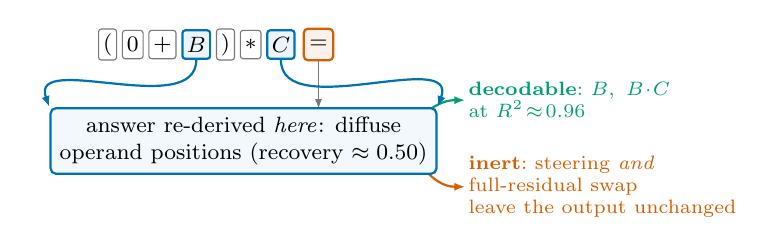
\begin{tikzpicture}[
  font=\footnotesize,
  tok/.style={draw=cbGray,rounded corners=1pt,minimum height=3.6mm,inner sep=1.6pt},
  op/.style={tok,draw=cbBlue,thick,fill=cbBlue!8},
  eq/.style={draw=cbOrange,thick,rounded corners=1.5pt,fill=cbOrange!8,minimum height=4mm,inner sep=2pt},
  probe/.style={-{Latex[length=1.4mm]},cbGreen,thick},
  dead/.style={-{Latex[length=1.4mm]},cbOrange,thick},
  comp/.style={-{Latex[length=1.4mm]},cbBlue,thick},
  lbl/.style={inner sep=1pt,font=\scriptsize},
]
% token row
\node[tok] (p1) {(};
\node[tok,right=0.6mm of p1] (z) {0};
\node[tok,right=0.6mm of z] (pl) {+};
\node[op,right=0.6mm of pl] (B) {$B$};
\node[tok,right=0.6mm of B] (p2) {)};
\node[tok,right=0.6mm of p2] (st) {$*$};
\node[op,right=0.6mm of st] (C) {$C$};
\node[eq,right=0.9mm of C] (eq) {$=$};

% residual node at '='
\node[draw=cbOrange,thick,rounded corners=2pt,fill=cbOrange!5,
      below=6mm of eq,minimum width=17mm,minimum height=5mm,align=center] (res)
      {answer-site\\ residual};
\draw[-{Latex[length=1.2mm]},cbGray] (eq) -- (res);

% probe (decodable)
\node[lbl,cbGreen,align=left,right=10mm of res,yshift=5mm] (dec)
     {\textbf{decodable}:\ $B,\ B\!\cdot\!C$\\ at $R^2\!\approx\!0.96$};
\draw[probe] (res.east) to[out=25,in=180] (dec.west);

% steering + swap (inert)
\node[lbl,cbOrange,align=left,right=10mm of res,yshift=-6mm] (dead)
     {\textbf{inert}:\ steering \emph{and}\\ full-residual swap\\ leave the output unchanged};
\draw[dead] (res.east) to[out=-25,in=180] (dead.west);

% computation route from operands
\node[draw=cbBlue,thick,rounded corners=2pt,fill=cbBlue!5,
      below=6mm of B,xshift=6mm,minimum width=30mm,minimum height=5mm,align=center] (route)
     {answer re-derived \emph{here}: diffuse\\ operand positions (recovery $\approx 0.50$)};
\draw[comp] (B.south) to[out=-90,in=110] (route.north west);
\draw[comp] (C.south) to[out=-90,in=70] (route.north east);
\end{tikzpicture}%
}
\caption{The answer-site subspace is \emph{dormant}, not missing. At the ``$=$''
position the operand and near-product are linearly decodable, but that direction is
causally inert (steering and a full-residual swap change nothing) and operand-explained;
the answer is instead re-derived diffusely from the operand positions. Decodability at
the answer site is not evidence of computation there.}
\label{fig:hero}
\end{figure}


\paragraph{Contributions.}
\begin{itemize}[topsep=2pt,itemsep=1pt,leftmargin=1.2em]
\item A token-matched, control-rich instance of a compositional arithmetic blind spot
in Llama-3.1-8B: operation-specific, depth-sensitive, magnitude-controlled, and
few-shot-recoverable, each with a confidence interval (\S\ref{sec:blindspot}).
\item Evidence that the decodable answer-site subspace is \emph{operand-dominated}:
it has no margin over a linear-$(B,C)$ baseline where the band leaves no headroom, and
only a small margin (gap $\approx 0.06$, CI excludes zero) where it does, robust to a
pre-registered probe layer (\S\ref{sec:dormant}).
\item A causal test showing the decodable direction is \emph{inert}: probe-direction
steering and a full-residual swap at the answer position both leave the output unchanged,
anchored by a positive control (the same-family patching moves the answer at the operand
positions, recovery $0.50$), so the null is a dead site, not a dead probe. Within the swap's
small sub-flip effect, $\approx 85\%$ of the variance is orthogonal to the decode direction
(\S\ref{sec:dormant}).
\item A cross-family replication in matched bare format, together with an explicit
prompt-format confound that we argue precludes reading the cross-model results as a
clean family dissociation (\S\ref{sec:generality}).
\end{itemize}

We read the answer-site subspace as \emph{dormant} in the sense of
\citet{makelov-etal-2024-subspace}: present to a probe, invisible to the computation.

\section{Related Work}
\label{sec:related}

\paragraph{Surface form and mathematical brittleness.}
Model math accuracy is sensitive to surface structure that leaves the answer invariant.
\citet{williamson-etal-2025-syntactic}, at the same venue, characterize a behavioral blind spot
in natural-language word problems where failure tracks dependency-locality complexity and
recovers under structure-lowering rephrasing, and conjecture a coupling between surface form and
internal representation. Our instance is orthogonal on both axes and \emph{tests} that
conjecture: a token-matched \emph{symbolic} expression whose additive-identity wrapper carries no
dependency-locality cost, for which we show the obvious representational reading (a
computed-but-unused product at the answer site) does not hold; the internal signature is a
dormant, operand-explained subspace, not a missing representation. \citet{reusch-lehner-2022-extracting}
show operator-tree structure is decodable from embeddings; we show that answer-site decodability
of the arithmetic \emph{value} can be an operand-reconstructible artifact that is causally inert,
so decodability of arithmetic structure does not certify its use.

\paragraph{Decodability versus causal use.}
A linear probe measures correlation, not use \citep{belinkov-2022-probing}, and can succeed on
random labels without a control \citep{hewitt-liang-2019-designing}. The sharpest form is the
subspace-patching illusion of \citet{makelov-etal-2024-subspace}: a direction can carry a
decodable signal yet be causally disconnected from the output. Our result is an arithmetic
instance of this illusion, established with a baseline and a steering test rather than assumed.
\citet{matsumoto-etal-2022-tracing} find decoded intermediate values in neural math solvers to
be causally usable; we find a decodable answer-site subspace that is causally inert. The results
are compatible: whether a decodable value is used is a per-site empirical question.

\paragraph{Mechanisms of arithmetic.}
\citet{stolfo-etal-2023-mechanistic} trace arithmetic from operand tokens to the final position
through late modules, and \citet{nikankin-etal-2025-arithmetic} argue models use a diffuse ``bag
of heuristics.'' Our localization agrees, and adds that the decodable answer-site value, easily
mistaken for the computed result, is a byproduct of that operand information. For method we
follow patching best practice \citep{zhang-nanda-2024-towards, heimersheim-nanda-2024-use}:
symmetric counterfactuals, a full-answer log-probability metric, and a positive control per null.

\section{Setup and Research Questions}
\label{sec:setup}

\paragraph{Model and stimuli.}
We study Llama-3.1-8B \citep{grattafiori-etal-2024-llama}, base and instruction-tuned, in bare
continuation format, by greedy decoding and integer parsing. Stimuli are $N = 400$ operand pairs
$(B, C)$ drawn once with a fixed seed from $[20, 49]$ and held constant across every condition,
token-length matched, with spacing controlled. The central contrast is
$\text{C1} = (\,0 + B\,) * C =$ (the composed failure) against $\text{C4} = (\,B * C\,) =$
(multiply inside a bracket, succeeds) and $\text{C6} = (\,0 + B\,) =$ (evaluate the wrapper,
succeeds).

\paragraph{Metrics.}
Accuracies carry Wilson intervals; paired contrasts carry paired bootstrap intervals
(10{,}000 resamples). Decodability is five-fold cross-validated ridge $R^2$ (item-bootstrap
interval; selectivity-gap CIs use 300 resamples given the per-draw cross-validation cost) at a
named token position. Selectivity compares the decode against a linear-$(B,C)$
baseline (a probe given only the raw operands and Gaussian noise), so a high $R^2$ that is
merely linear in the operands does not count as representing the product. Causal tests use
symmetric operand counterfactuals and a full-answer log-probability metric
$\Delta = \log p(P') - \log p(\text{true})$; because Llama chunks the leading digits, a
first-token score is non-discriminative between two products.

\paragraph{Research questions.} \textbf{RQ1}: is the composition failure a genuine, controlled
effect or an artifact of difficulty, magnitude, or elicitation (\S\ref{sec:blindspot})?
\textbf{RQ2}: is the near-product decodable at the answer site a \emph{represented} quantity or
reconstructible from the operands alone (\S\ref{sec:dormant})? \textbf{RQ3}: is the decodable
direction causally used to produce the answer (\S\ref{sec:dormant})?

\section{The Blind Spot}
\label{sec:blindspot}

\begin{table}[t]
\centering
\footnotesize
\setlength{\tabcolsep}{3.2pt}
\begin{tabular}{@{}llcc@{}}
\toprule
 & surface & base & instruct \\
\midrule
C0 & \texttt{B * C =} & 0.838 & 0.848 \\
C4 & \texttt{( B * C ) =} & 0.890 & 0.908 \\
C6 & \texttt{( 0 + B ) =} & 1.000 & 1.000 \\
\textbf{C1} & \texttt{( 0 + B ) * C =} & \textbf{0.508} & \textbf{0.265} \\
A1 & \texttt{( 0 + B ) + C =} & n/a & 0.995 \\
D1 & \texttt{(( 0 + B )) * C =} & n/a & 0.038 \\
\bottomrule
\end{tabular}
\caption{The composition blind spot (exact-match accuracy, $N{=}400$). The parts succeed
(C4, C6) but the composition collapses (C1); $\Delta(\text{C4}{-}\text{C1}) = 0.64$, CI
$[.60,.69]$ (instruct). A1/D1 are instruct-only. Full battery with Wilson intervals in
Appendix~\ref{app:battery}.}
\label{tab:battery}
\end{table}

The model evaluates every ingredient of $(\,0 + B\,) * C$ yet fails to compose them
(Table~\ref{tab:battery}). We establish that this is a real effect, not an artifact,
with four controls, and we state each at the precision the data support.

\paragraph{It is operation-specific, not format brittleness.} Replacing the outer
multiplication with addition, $(\,0 + B\,) + C =$, restores accuracy to $0.995$ (instruct)
against $0.265$ under \emph{identical} format; $\Delta(\text{A1}-\text{C1}) = 0.730$, $95\%$ CI
$[0.69, 0.77]$. It is also spacing-invariant: with all spaces removed the inside-bracket
multiply still survives (C8 $= 0.785$ instruct, $0.765$ base) while the composition still
collapses (C7 $= 0.19$, $0.018$), the same dissociation. So it is not generic spacing or
parenthesis sensitivity; specifically the multiplicative composition breaks. (A1/A2 are
instruct-only; we do not extrapolate to base.)

\paragraph{It is controlled, not an artifact.} Three further controls hold. \emph{Depth} is
a distinct stressor: a redundant nesting $(\,(\,0 + B\,)\,) * C =$ drops to $0.038$, but
nesting degrades \emph{addition} too (nested addition $0.665$, base), so we treat depth as a
general parsing stressor, not more composition evidence. \emph{Magnitude} is ruled out: within
every matched-$|B\!\cdot\!C|$ bin C1 stays well below C4 ($0.53$ vs $0.96$ smallest, $0.00$ vs
$0.70$ largest). And the collapse is an \emph{elicitation} fragility: two to four fixed-seed
in-context examples recover C1 to the C4 ceiling (instruct $0.265 \to 0.885\,{\scriptsize[.85,.91]}
\to 0.915\,{\scriptsize[.88,.94]}$; base $0.508 \to 0.838 \to 0.882$), so it is not an inability
to multiply.

\paragraph{Two overstatements we avoid.} The effect is neither universal (base $(\,B + 0\,) * C$
barely moves, drop $0.015$, vs $0.33$ for $(\,0 + B\,)$; Appendix~\ref{app:wrapper}) nor
uniformly worse under tuning (on plain parentheses instruct is \emph{better}, $0.755$ vs
$0.495$); and C0, not $1.0$, is the reference ceiling ($B * C =$ is $0.848$ instruct).

\section{A Dormant Subspace}
\label{sec:dormant}

\begin{figure*}[t]
\centering
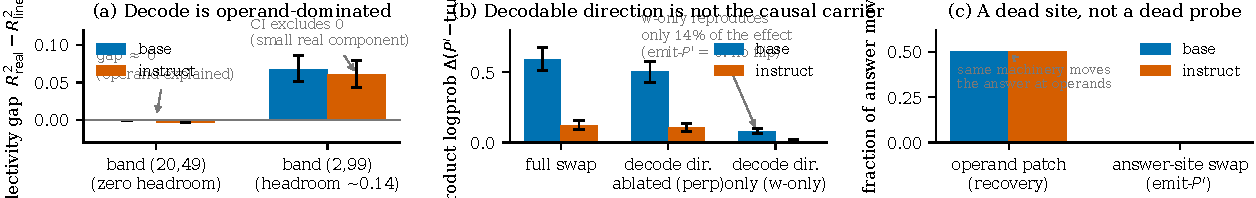
\includegraphics[width=0.82\textwidth]{figs/fig2_evidence.pdf}
\caption{The decodable answer-site subspace is dormant (bars/error bars are $95\%$ CIs).
\textbf{(a)} Selectivity gap (decode $R^2$ for \bc{} at ``$=$'' minus a linear-$(B,C)$ baseline):
at $[20,49]$ no headroom (gap $\approx 0$, operand-explained); at $[2,99]$ a small gap whose CI
excludes zero. \textbf{(b)} Causal share of a full-residual swap at the C4 ``$=$'' (base): ablating
the decode direction (perp) preserves most of the effect, the decode direction alone (w-only)
reproduces little, CIs non-overlapping; the swap flips no answers (emit-$P' = 0$). \textbf{(c)} The
dissociation as a fraction of the answer moved (two metrics): patching moves the answer at the
operand positions (recovery $0.50$) but the answer-site swap flips nothing, a dead \emph{site}, not
a dead probe. \textbf{(d)} Inject dose-response on the same axis: the C1 claim site is flat at
every dose (CIs bracket 0) while the C4 reference rises monotonically (base) yet never flips;
instruct's reference is weak and non-monotone.}
\label{fig:evidence}
\end{figure*}

The seductive story is that the product is computed and represented at the answer position but
not read out. We test it in three steps and reject it.

\paragraph{The product decodes (RQ2, correlational).}
A cross-validated probe recovers \bc{} from the ``$=$'' residual at $R^2 = 0.965$ (instruct),
$0.967$ (base) and the operand $B$ at $0.96$--$0.97$, with $B$ decodable at ``)'' at \emph{every} layer
including the last (instruct $0.98$, layer 31); taken alone this looks like a represented product.

\paragraph{But the decode is operand-dominated (RQ2, selectivity).}
Decodability of \bc{} need not mean the product is represented, since \bc{} is itself largely
linear in $B, C$ over a narrow band. We test this with a selectivity gap over a linear-$(B,C)$
baseline, but the gap test only has resolving power when the baseline leaves headroom:

\begin{proposition}[Headroom bound]
\label{prop:headroom}
For a target $g$, a decode probe with cross-validated $R^2_{\mathrm{real}}\le 1$, and a baseline
feature class $F$ with cross-validated $R^2_{F}$ on distribution $D$, the selectivity gap obeys
$\mathrm{gap}=R^2_{\mathrm{real}}-R^2_{F}\le 1-R^2_{F}$. The gap test therefore resolves at most the
\emph{headroom} $1-R^2_{F}$, so headroom is a design statistic that must be reported.
\end{proposition}

\noindent (Proof in Appendix~\ref{app:proof}; it applies to any derived quantity nearly linear in
its inputs on-distribution.) We compare \bc{} against the linear-$(B,C)$ baseline
(Figure~\ref{fig:evidence}a). At $[20,49]$ the baseline reaches $R^2 = 0.968$: by
Prop.~\ref{prop:headroom} the headroom is only $0.032$, so the test is a priori near-vacuous, and
indeed the gap is $-0.0002$. At $[2,99]$, where \bc{} is nonlinear in the operands (headroom
$0.135$), a small gap appears: $+0.068$, $95\%$ CI $[0.051, 0.086]$
(base) and $+0.060$, $[0.043, 0.079]$ (instruct), both excluding zero, and still positive at a
layer chosen by a C1-independent criterion (the C4 decode peak) rather than the C1 argmax. We flag that $[2,99]$ is
a harder regime where the parts fall below our $0.80$ floor (C4 $= 0.71$ base,
$0.73$ instruct), so we read it as a stress test, not a comfortably
in-scope measurement, and rest the headline on the band-independent causal null below. The
decode is operand-dominated ($\geq 0.94$ of it is reproduced by the linear-$(B,C)$ baseline,
$\approx 1.0$ at $[20,49]$) with at most a small operand-nonlinear component, consistent with a
weak product signal (behavior-tracking: C4 gap $>$ C1 gap, difference CI excludes zero).

\paragraph{And the decodable direction is causally inert (RQ3).}
We steer the ``$=$'' residual along the fitted direction to write a counterfactual product $P'$,
on held-out items. On the first-token metric the inject is null at every layer and matches
norm-matched random and shuffled controls (Appendix~\ref{app:steering}), but that metric is
non-discriminative between products. On the discriminative full-product metric, injecting at the
C1 ``$=$'' is flat at every dose $k \in \{1,2,4,8\}$ (CIs bracket zero) while the same inject at
the succeeding C4 ``$=$'' rises monotonically ($+0.08 \to +0.46$, every CI excluding zero, base)
yet never flips: the axis has dynamic range where the product is used and none at the failing
site, a dead direction rather than a dead instrument (emit-$P'$ stays zero throughout, a
saturating criterion, so we read the log-probability). A full-residual swap at the C4 ``$=$'',
\emph{where the model succeeds}, likewise fails to transplant the donor product (emit-$P' = 0$;
log-probability $+0.59$ at L19 where we decompose it, peak $+0.66$ at L23, still sub-flip); after
the swap the model still emits its \emph{own} correct answer at $0.90$--$0.95$ across L19--L31, so
the site is demonstrably bypassed. The product is thus not linearly resident at ``$=$'' even where
computed correctly, a fortiori at C1.
The one intervention that moves the answer is at the operand positions (recovery $0.50$; a
clean-answer recovery metric, a different readout and operation).

\paragraph{Certifying the illusion.}
We decompose the C4 swap effect into the decode direction and its orthogonal complement
(Figure~\ref{fig:evidence}b). Ablating the decode direction still leaves $+0.50$ (base), while
the decode direction alone contributes only $+0.08$, with non-overlapping CIs: $\approx 85\%$ of
the swap's (sub-flip) answer-effect survives removing the decodable direction (the swap moves only
$\approx 20\%$ of its magnitude along it). (The instruct swap effect is smaller, $+0.12$, its
decode-direction component not significantly positive; we report the decomposition for base.) We
use \emph{dormant} strongly: unlike a patch-potent-but-unused component, this direction moves
essentially nothing even when patched, present to a probe but invisible to computation
\citep{makelov-etal-2024-subspace}. Consistent with \citet{stolfo-etal-2023-mechanistic}
and \citet{nikankin-etal-2025-arithmetic}, the operands carry the signal but no sparse head set
reconstructs it (best head $< 0.02$); the value at ``$=$'' decodes and correlates yet cannot be
steered.

\paragraph{As a causal-abstraction claim.}
The full-residual swap is an interchange intervention \citep{geiger-etal-2021-causal} on the
``$=$'' residual: substituting a donor's representation should, if $B\!\cdot\!C$ is computed and
stored there, install the donor's answer. Interchange accuracy is $0$ (emit-$P'=0$) and the
original answer survives (emit-true $0.90$--$0.95$), so the hypothesis ``\bc{} is computed at
(``$=$'', layer $l$)'' fails as a causal-abstraction claim at every late $l$, even though the
correlational decode holds. Decodability and causal realization come apart at this node.

\paragraph{Hypotheses and evidence.}
Table~\ref{tab:hyp} collects the three readings of the failure against the committed evidence.

\begin{table}[t]
\centering
\footnotesize
\setlength{\tabcolsep}{3pt}
\begin{tabular}{@{}p{2.35cm}p{1.15cm}p{3.1cm}@{}}
\toprule
Hypothesis & Verdict & Evidence (committed) \\
\midrule
H1: product \emph{stored} at ``$=$'' & rejected & swap emit-$P'{=}0$, dose C1 flat, emit-true $0.90$--$0.95$ \\
H2: \emph{assembled} at readout from operands & supported & operand recovery $0.50$; $B$ decodable at every layer incl.\ 31; emit-true $0.90$--$0.95$ \\
H3: sparse answer-site circuit & no locus & best head $<0.02$; all heads inconclusive \\
\bottomrule
\end{tabular}
\caption{The composition failure adjudicated. Every cell traces to a committed file
(Appendix~\ref{app:battery}; \texttt{lateswap}, \texttt{dose\_response},
\texttt{operand\_localization}, \texttt{position\_decodability}, \texttt{head\_path\_patch}).}
\label{tab:hyp}
\end{table}

\paragraph{Predictions.}
H2 is falsifiable. It predicts that (i) ablating attention from ``$=$'' to the operand positions
during generation should destroy C4 accuracy, and (ii) few-shot recovery should act at the operand
positions rather than at ``$=$''. We state these as predictions, not results.

\section{Generality and Limitations}
\label{sec:generality}

\paragraph{Replication in matched format, and a format confound.}
In matched bare format the collapse is not specific to Llama-3.1-8B. Among models that clear a
parts floor (C4, C6 $\geq 0.80$), the composed form collapses for Gemma-2-9b-it (C1 $= 0.043$,
C4 $= 0.99$) and Llama-3.2-3B (C1 $= 0.36$), alongside base and instruct Llama-3.1-8B; three
others fail the parts in bare format and are out of scope, not counterexamples
(Appendix~\ref{app:crossmodel}). Chat formatting changes this, not
cleanly: Gemma-2-9b-it \emph{composes} in its native chat template (C1 $= 0.95$), but there
Llama-3.1-8B falls below the parts floor (C4 $= 0.70$)
and leaves scope, so the composing and failing models are never compared in the same format. We
read this as replication in matched bare format plus a prompt-format confound, \emph{not} as
evidence that some families are immune; per-model native-format evaluation is the right axis for
a clean cross-family claim, which we do not make.

\paragraph{Limitations.}
The causal localization is distributed (operand positions matter but no sparse circuit is
recovered), so we characterize \emph{where}, not a minimal mechanism; the operation and depth
controls are instruct-only; and the zero-excluding gap is small and only in the harder band, with
the dormancy resting on the causal-share certification. None of these affects the central result.

\paragraph{Conclusion.}
A parenthesized additive identity selectively breaks multiplicative composition in Llama-3.1-8B,
and the ``represented but unused'' reading of the decodable answer site is an illusion: it is
operand-dominated and causally inert, so a high decodability $R^2$ needs a baseline and a causal
control before it licenses a mechanistic claim.


\bibliography{refs}

\appendix
\section{Full Battery and Confidence Intervals}
\label{app:battery}

Table~\ref{tab:fullbattery} gives every condition with Wilson $95\%$ intervals
($N = 400$). Base A1/A2/D1 are not in our committed data and are omitted rather than
estimated.

\begin{table}[h]
\centering
\footnotesize
\setlength{\tabcolsep}{3pt}
\begin{tabular}{@{}llcc@{}}
\toprule
 & surface & base & instruct \\
\midrule
C0 & \texttt{B * C =} & .838\,{\scriptsize[.80,.87]} & .848\,{\scriptsize[.81,.88]} \\
C1 & \texttt{( 0 + B ) * C =} & .508\,{\scriptsize[.46,.56]} & .265\,{\scriptsize[.22,.31]} \\
C2 & \texttt{( 0 + B * C ) =} & n/a & .678\,{\scriptsize[.63,.72]} \\
C3 & \texttt{( B ) * C =} & n/a & .755\,{\scriptsize[.71,.80]} \\
C4 & \texttt{( B * C ) =} & .890\,{\scriptsize[.86,.92]} & .908\,{\scriptsize[.88,.93]} \\
C5 & \texttt{0 + B * C =} & n/a & .542\,{\scriptsize[.49,.59]} \\
C6 & \texttt{( 0 + B ) =} & 1.00\,{\scriptsize[.99,1.0]} & 1.00\,{\scriptsize[.99,1.0]} \\
C7 & \texttt{(0+B)*C=} & .018\,{\scriptsize[.01,.04]} & .190\,{\scriptsize[.16,.23]} \\
C8 & \texttt{(B*C)=} & .765\,{\scriptsize[.72,.80]} & .785\,{\scriptsize[.74,.82]} \\
A1 & \texttt{( 0 + B ) + C =} & n/a & .995\,{\scriptsize[.98,1.0]} \\
A2 & \texttt{0 + ( B + C ) =} & n/a & .928\,{\scriptsize[.90,.95]} \\
D1 & \texttt{(( 0 + B )) * C =} & n/a & .038\,{\scriptsize[.02,.06]} \\
\bottomrule
\end{tabular}
\caption{Full battery, exact-match accuracy with Wilson $95\%$ CIs.}
\label{tab:fullbattery}
\end{table}

\paragraph{Magnitude control.} Within matched $|B\!\cdot\!C|$ bins (instruct), C1 vs C4:
$[440,813)$ .53/.96 ($n{=}79$); $[813,1185)$ .28/.94 (126); $[1185,1558)$ .16/.89 (104);
$[1558,1930)$ .19/.89 (64); $[1930,2303)$ .00/.70 (27). Every paired difference has a
positive bootstrap CI.

\section{Wrapper Blind-Spot Map}
\label{app:wrapper}
\begin{figure}[h]
\centering
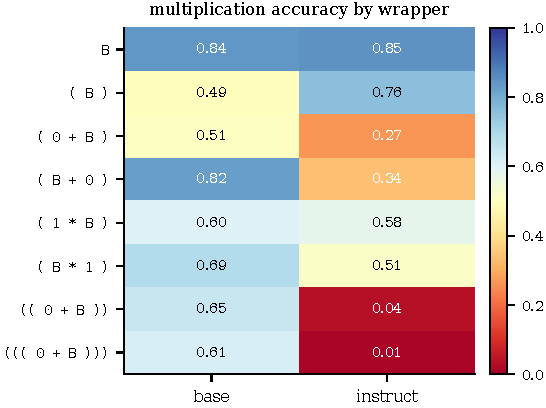
\includegraphics[width=0.82\columnwidth]{figs/figA_wrapper.pdf}
\caption{Multiplication accuracy by wrapper. Position-dependence is a base-model effect
(left-placed $(\,0{+}B\,)$ collapses, right-placed $(\,B{+}0\,)$ barely moves; instruct degrades
on both placements), and instruction tuning is not uniformly worse (plain parentheses).}
\label{fig:wrapper}
\end{figure}

\section{By-Layer Decodability}
\label{app:decode}
\begin{figure}[h]
\centering
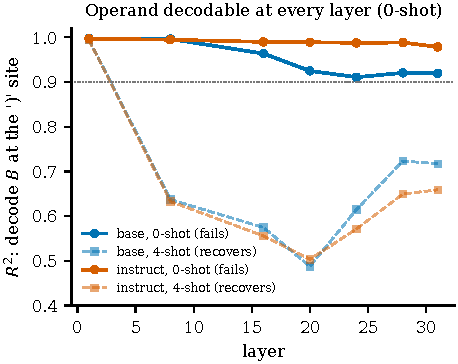
\includegraphics[width=0.82\columnwidth]{figs/figA_decode.pdf}
\caption{Operand $B$ decodes at every layer in the failing zero-shot regime (solid). The
few-shot curves (dashed) drop mid-network; shown for completeness only, and we draw no
mechanistic conclusion from the few-shot decodability.}
\label{fig:decode}
\end{figure}

\section{Steering Nulls}
\label{app:steering}
\begin{figure}[h]
\centering
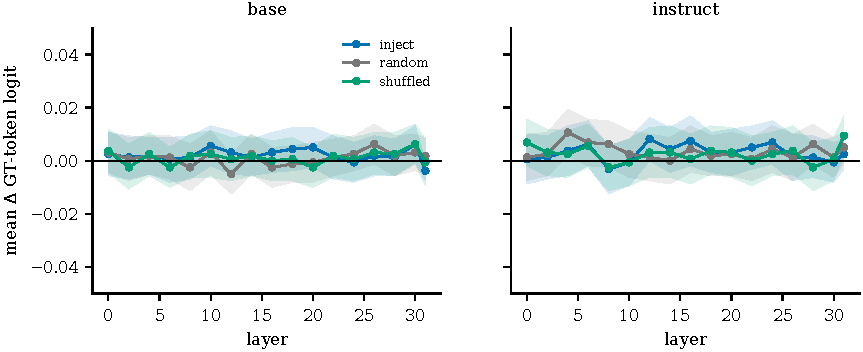
\includegraphics[width=\columnwidth]{figs/figA_steering.pdf}
\caption{Probe-direction steering at ``$=$'' is inert at every layer for inject, random,
and shuffled targets (mean $\Delta$ ground-truth-token logit, $95\%$ CIs through zero).
This first-token metric is a null; the discriminative full-product re-score is
Figure~\ref{fig:evidence}b.}
\label{fig:steernull}
\end{figure}

\section{Cross-Model Battery}
\label{app:crossmodel}
Matched bare format, in scope if C4 and C6 $\geq 0.80$: Llama-3.1-8B base C1 $.508$ /
instruct $.265$; Gemma-2-9b-it $.043$ (C4 $.99$); Llama-3.2-3B $.358$ (C4 $.88$). Out of
scope (parts fail): Qwen2.5-7B (C4 $.00$), Mistral-7B (C4 $.62$), Llama-3.2-1B (C4 $.31$).
Chat format: Gemma-2-9b-it composes (C1 $.95$, C4 $.99$) but Llama-3.1-8B chat falls out of
scope (C4 $.70$); the composing and failing models are never in the same format.


\end{document}
